





\documentclass{beamer}
%  \usepackage[utf8]{inputenc}
\usepackage[utf8]{inputenc}
  \usetheme{Warsaw}
  \usepackage{dsfont}
  \usepackage{xcolor}
%  \usepackage[dvipsnames]{xcolor}
  \usepackage{tabto}

\usepackage{mathtools}
\usepackage{todonotes}
\usepackage{microtype}

\usepackage{complexity}
\usepackage{amsmath}

\usepackage{stmaryrd}
\usepackage{dsfont}



\usepackage{mathrsfs}
\usepackage{mathalpha}
\usepackage{amsmath}
\usepackage{amsfonts}
\usepackage{multirow}

\usepackage{ textcomp } 

\usepackage{stmaryrd}
\usepackage{wrapfig}


\title[Resilience and Home-Space for WSTS]{Resilience and Home-Space for WSTS}

\author[Alain Finkel ~ Mathieu Hilaire]{Alain Finkel \inst{1} \and Mathieu Hilaire \inst{2}}
\institute[Alain Finkel ~ Mathieu Hilaire]{\inst{1} Université Paris-Saclay, CNRS, ENS Paris-Saclay, LMF, Gif-sur-Yvette, France, Institut Universitaire de France \and %
                      \inst{2} Université Lyon 1, LIRIS, France}

\date{}





\usepackage{pgf}
\usepackage{tikz}
\usetikzlibrary{arrows,automata}
%\usepackage[latin1]{inputenc}

\bibliographystyle{alpha}% the recommnded bibstyle

\newcommand{\Z}{\mathbb{Z}}
\newcommand{\N}{\mathbb{N}}


\colorlet{Mycolor1}{green!10!orange!90!}
\colorlet{Mycolor3}{blue!20!magenta!90!}
\definecolor{Mycolor2}{HTML}{00F9DE}


\newcommand{\pred}{\textsf{pred}}
\newcommand{\post}{\textsf{post}}



\newcommand{\Bad}{\textsf{Bad}}
\newcommand{\Safe}{\textsf{Safe}}


\begin{document}


\maketitle


%vvvvvvvvvvvvvvvvvvvvvvvvvvvvvvvvvvvvvvvvvvvvvvvvvvvvvvvvvvvvvvvvvvvvvvvvvv
  \begin{frame}{Outline}

\tableofcontents
  \end{frame}
  \section{Introduction}
%vvvvvvvvvvvvvvvvvvvvvvvvvvvvvvvvvvvvvvvvvvvvvvvvvvvvvvvvvvvvvvvvvvvvvvvvvv
  \begin{frame}{Motivation}

\begin{columns}[T]
 \column{0.35\textwidth}
 \begin{figure}
 	\hspace{-0.5cm}

\includegraphics[width=1.\textwidth]{fridge}
% \caption{Hasse diagram of some classes of transition systems, together with the decidability (in green) or undecidability (in red) of the resilience problems. Decidability of bounded resilience and $k-$resilience variants are indicated in blue.}
\end{figure} 

 \column{0.65\textwidth}
\phantom{Fridge.png} \\
{\sf Bad} state is when temperature is too high \\
 {\sf Good} state is temperature low enough \\

\end{columns}

\pause

\phantom{Fridge.png} \\
Other applications e.g. refrigerating medical supplies or nuclear reactor 

\iffalse
  \todo[inline,color=blue!20]{ {\it À l'oral~}
We are usually focused on how to avoid bad states in general but you can see when your fridge the system stops providing refrigerating temperature it's not over yet
If you leave your fridge off for a minute it's not going to have Terrible impact but if you leave it off for more than one hour you're gonna have to throw the things in it away

And I've been talking like your frige at home but it apply to any type of cooling system it can be like refrigerating medical supplies or nuclear reactor.

And this is interesting Bcz now the stuff is not necessarily avoid bad states completely

This lead to concept of resilience
}
\fi

  \end{frame}
%vvvvvvvvvvvvvvvvvvvvvvvvvvvvvvvvvvvvvvvvvvvvvvvvvvvvvvvvvvvvvvvvvvvvvvvvvv
  \begin{frame}{Example}
  
  
   \begin{center}
 	\begin{figure}
 	\vspace{.06cm}
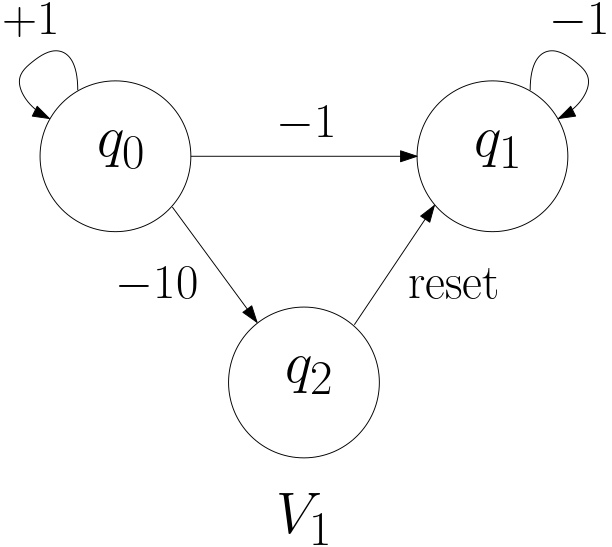
\includegraphics[width=.50\textwidth]{FigA}
	\end{figure}
\end{center}  

  \end{frame}
%vvvvvvvvvvvvvvvvvvvvvvvvvvvvvvvvvvvvvvvvvvvvvvvvvvvvvvvvvvvvvvvvvvvvvvvvvv
  \begin{frame}{Example}
  
  
   \begin{center}
 	\begin{figure}
% 	\hspace{-2.cm}
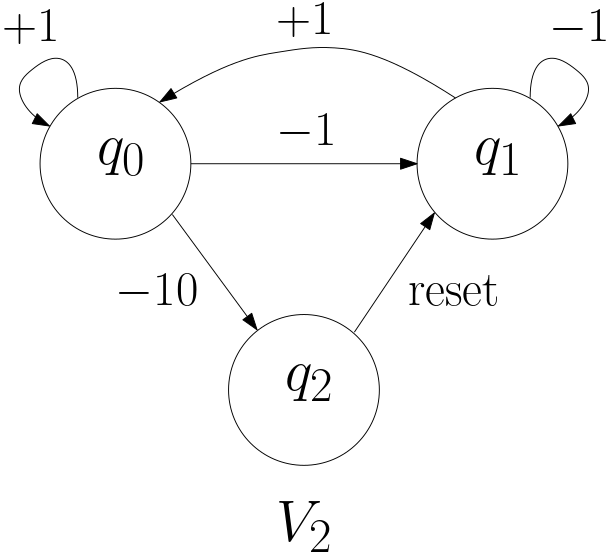
\includegraphics[width=.50\textwidth]{FigB}
	\end{figure}
\end{center}  

  \end{frame}
%vvvvvvvvvvvvvvvvvvvvvvvvvvvvvvvvvvvvvvvvvvvvvvvvvvvvvvvvvvvvvvvvvvvvvvvvvv
  \begin{frame}{Resilience(s)}
  

% TODO

% Define the Six different problems we study/focus on.

% (Takes some room but I think mb having the six on the same page could be better than having three then three state-* on two separate pages ?)
  
 {\small
  
  
{\sc Resilience problems}

\hspace{-0.5cm}  {\bf INPUT:\ }{A transition system $\mathscr{S}=(S,\rightarrow)$, and a set $\Safe \subseteq S$.}

\hspace{-0.5cm}  {\bf QUESTION:\ }{ ({\sc resilience problem (RP)}) $\Bad \rightarrow^{*} \Safe$ ?

\hspace{-0.5cm}  ({\sc $k$-resilience problem (kRP)})		$\Bad \rightarrow^{\leq k} \Safe$ ?

\hspace{-0.5cm}  ({\sc bounded resilience problem (BRP)})	$\exists k ~ S \rightarrow^{\leq k} \Safe$ ?\newline}

}

  \end{frame}
%vvvvvvvvvvvvvvvvvvvvvvvvvvvvvvvvvvvvvvvvvvvvvvvvvvvvvvvvvvvvvvvvvvvvvvvvvv
  \begin{frame}{Resilience(s)}
  
 {\small
 
  \hspace{-0.2cm}
{\sc \textcolor{red}{State} resilience problems}

\hspace{-0.5cm}  {\bf INPUT:\ }{A transition system $\mathscr{S}=(S,\rightarrow)$, \textcolor{red}{$s \in S$}, and a set $\Safe \subseteq S$.}

\hspace{-0.5cm}  {\bf QUESTION:\ }

\hspace{-0.5cm}{ ({\sc state-resilience problem (SRP)}) $\textcolor{red}{\post^*(s) } \rightarrow^{*} \Safe$ ?

\hspace{-0.5cm}  ({\sc $k$-state-resilience problem (kSRP)})		$\textcolor{red}{\post^*(s)} \rightarrow^{\leq k} \Safe$ ?

\hspace{-0.5cm} ({\sc bounded-state-resilience problem (BSRP)})	$\exists k ~ \textcolor{red}{\post^*(s)} \rightarrow^{\leq k} \Safe$?\newline}

 }

% \todo[inline,color=blue!20]{{\bf  \tiny (Takes some room but I think mb having the six on the same page could be better than having three then three state-* on two separate pages ?)}} 


  \end{frame}
%vvvvvvvvvvvvvvvvvvvvvvvvvvvvvvvvvvvvvvvvvvvvvvvvvvvvvvvvvvvvvvvvvvvvvvvvvv
	\section{Definitions}
  \begin{frame}{WSTS}
  
% TODO
  
  \todo[inline,color=blue!20]{ {\it À l'oral~} 
Resilience(s) "obviously"  undecidable in general so restriction
$\to$
restriction already to WSTS
$\to$
so we need to define WSTS properly
}

\begin{definition}[Definition 3.10, \cite{DBLP:journals/iandc/Finkel90}]
A {\em Well-Structured Transition System} (WSTS)  $\mathscr{S}=(S, \rightarrow, \leq)$
is a transition system $(S, \rightarrow)$
equipped with a wqo ${\leq} \subseteq S \times S$ such that   
the transition relation $ \rightarrow$ is (upward) compatible with $\leq$, i.e., for all 
$s_1, t_1 , s_2 \in S$
	with $s_1 \leq s_2$  and $s_1 \rightarrow t_1$, there exists 
	$t_2 \in S$ with 
	$t_1 \leq t_2$ and $s_2 \rightarrow^{*} t_2$.
\end{definition}


\todo[inline,color=blue!20]{    \tiny
diapo 5: théorème: c'est indécidable dans le cas général des systèmes de transitions
diapo 5: déjà pour les bien structurés c'est indécidable
résilience indécidable pour les post effectif WSTS quelque soit safe clos par le haut ou par le bas
}


%  \todo[inline,color=blue!20]{    \tiny Definition right now is very formal for a slideshow, maybe make it less verbose? }

  \end{frame}
%vvvvvvvvvvvvvvvvvvvvvvvvvvvvvvvvvvvvvvvvvvvvvvvvvvvvvvvvvvvvvvvvvvvvvvvvvv
  \begin{frame}{... on effectivity}
  
TODO


... and effectivity as well



  \end{frame}
%vvvvvvvvvvvvvvvvvvvvvvvvvvvvvvvvvvvvvvvvvvvvvvvvvvvvvvvvvvvvvvvvvvvvvvvvvv
  \begin{frame}{WBTS Taxonomy}
  
   \begin{center}
 	\begin{figure}
% 	\hspace{-2.cm}
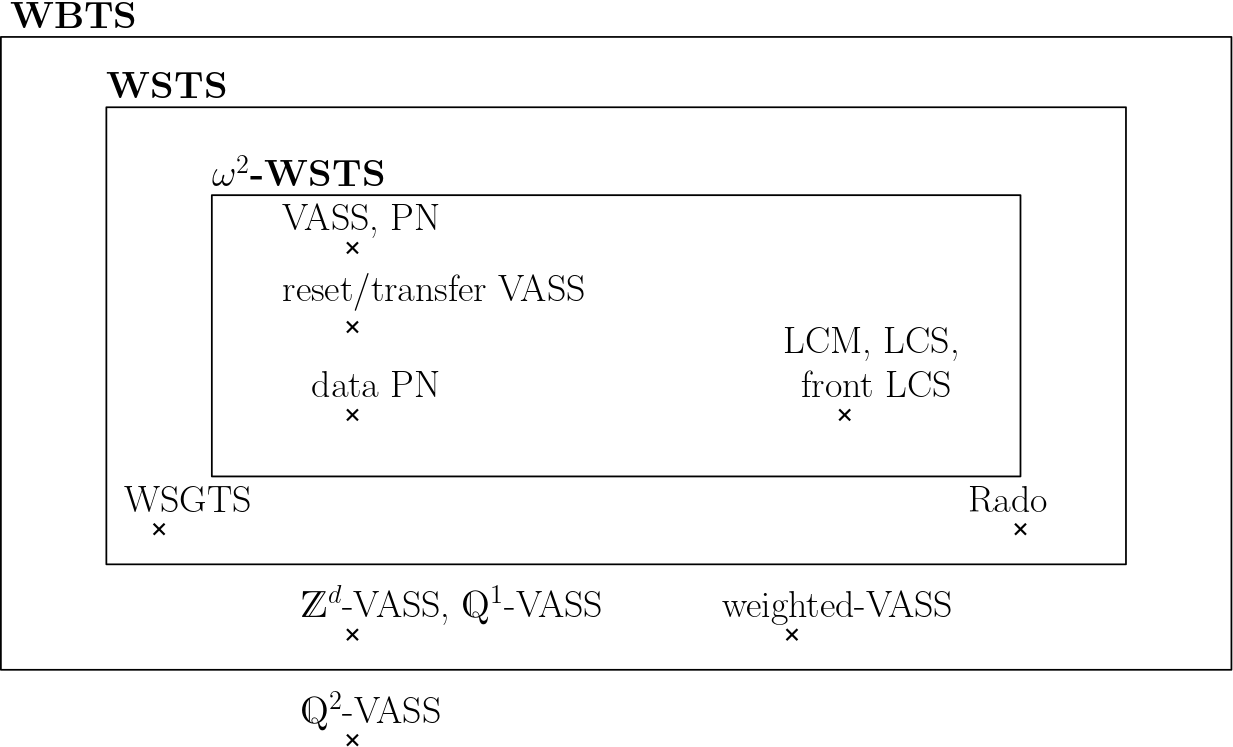
\includegraphics[width=.80\textwidth]{WSTS_taxonomy_large}
	\end{figure}
\end{center}  

  \todo[inline,color=blue!20]{ 
Refaire les références dans l'image (pas les même défintions/ref) 
}


  \end{frame}
%vvvvvvvvvvvvvvvvvvvvvvvvvvvvvvvvvvvvvvvvvvvvvvvvvvvvvvvvvvvvvvvvvvvvvvvvvv
  \begin{frame}{Results}
  
% Now that everything is somewhat properly defined maybe the picture with all the results ?  
  
   \begin{center}
 	\begin{figure}
 	\hspace{-2.cm}
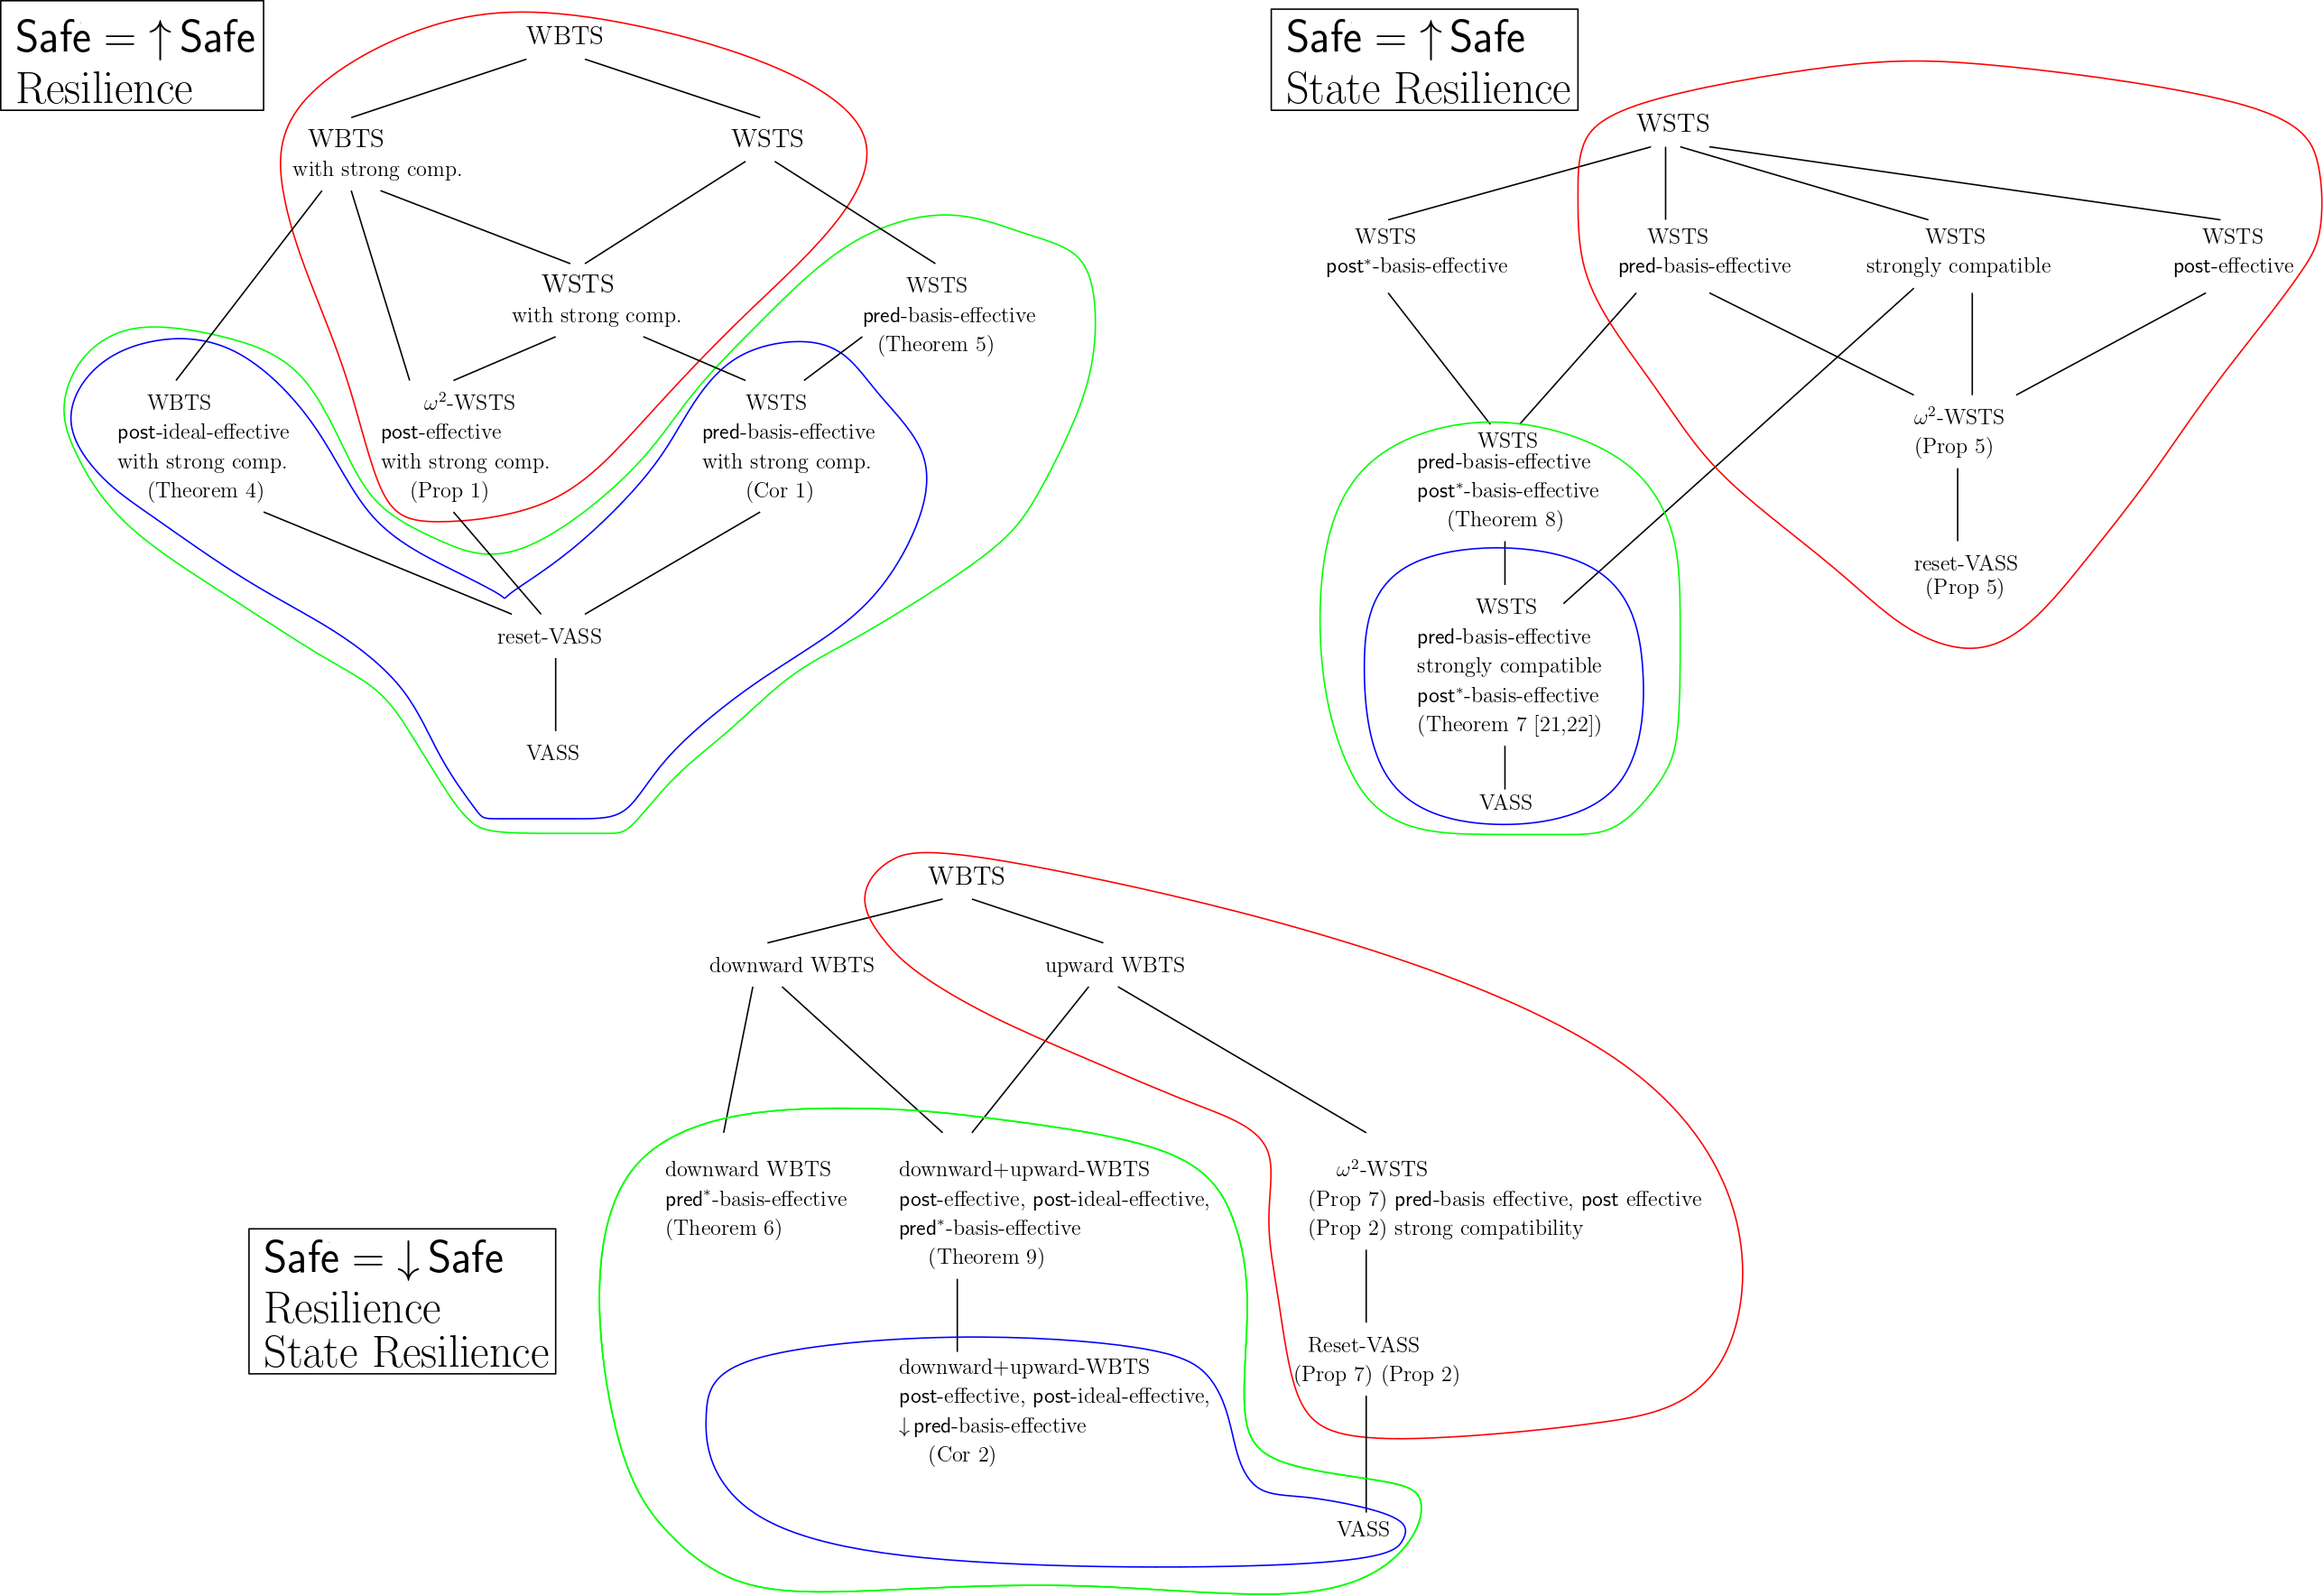
\includegraphics[width=1.00\textwidth]{All_results}
% \caption{Hasse diagram of some classes of transition systems, together with the decidability (in green) or undecidability (in red) of the resilience problems. Decidability of bounded resilience and $k-$resilience variants are indicated in blue.}
	\end{figure}
\end{center}  
    
  \end{frame}
%vvvvvvvvvvvvvvvvvvvvvvvvvvvvvvvvvvvvvvvvvvvvvvvvvvvvvvvvvvvvvvvvvvvvvvvvvv
  \begin{frame}{Result A}
 
  \todo[inline,color=blue!20]{ {\it À l'oral~} 
   Now we won't have time to detail all the result. 
}
   
  
   
Result A: Théorème 4 ou 5


\setcounter{theorem}{3}

\begin{theorem}\label{down-up}
Let $\mathscr{S}=(S,\rightarrow, \leq)$ be a $\post$-ideal-effective WBTS with strong compatibility and a set $\Safe = \mathop{\uparrow} \Safe$.
{\sc Resilience}, {\sc Bounded resilience} 
and {\sc $k$-resilience} are decidable.
\end{theorem}

ou

\begin{theorem}\label{xxx}
Let $\mathscr{S}=(S,\rightarrow, \leq)$ be a $\pred$-basis-effective WSTS and a set $\Safe = \mathop{\uparrow} \Safe$.
 {\sc Resilience} is decidable.
\end{theorem}

    
  \end{frame}
%vvvvvvvvvvvvvvvvvvvvvvvvvvvvvvvvvvvvvvvvvvvvvvvvvvvvvvvvvvvvvvvvvvvvvvvvvv
  \begin{frame}{Result A}
 
   \begin{center}
 	\begin{figure}
 	\hspace{-2.cm}
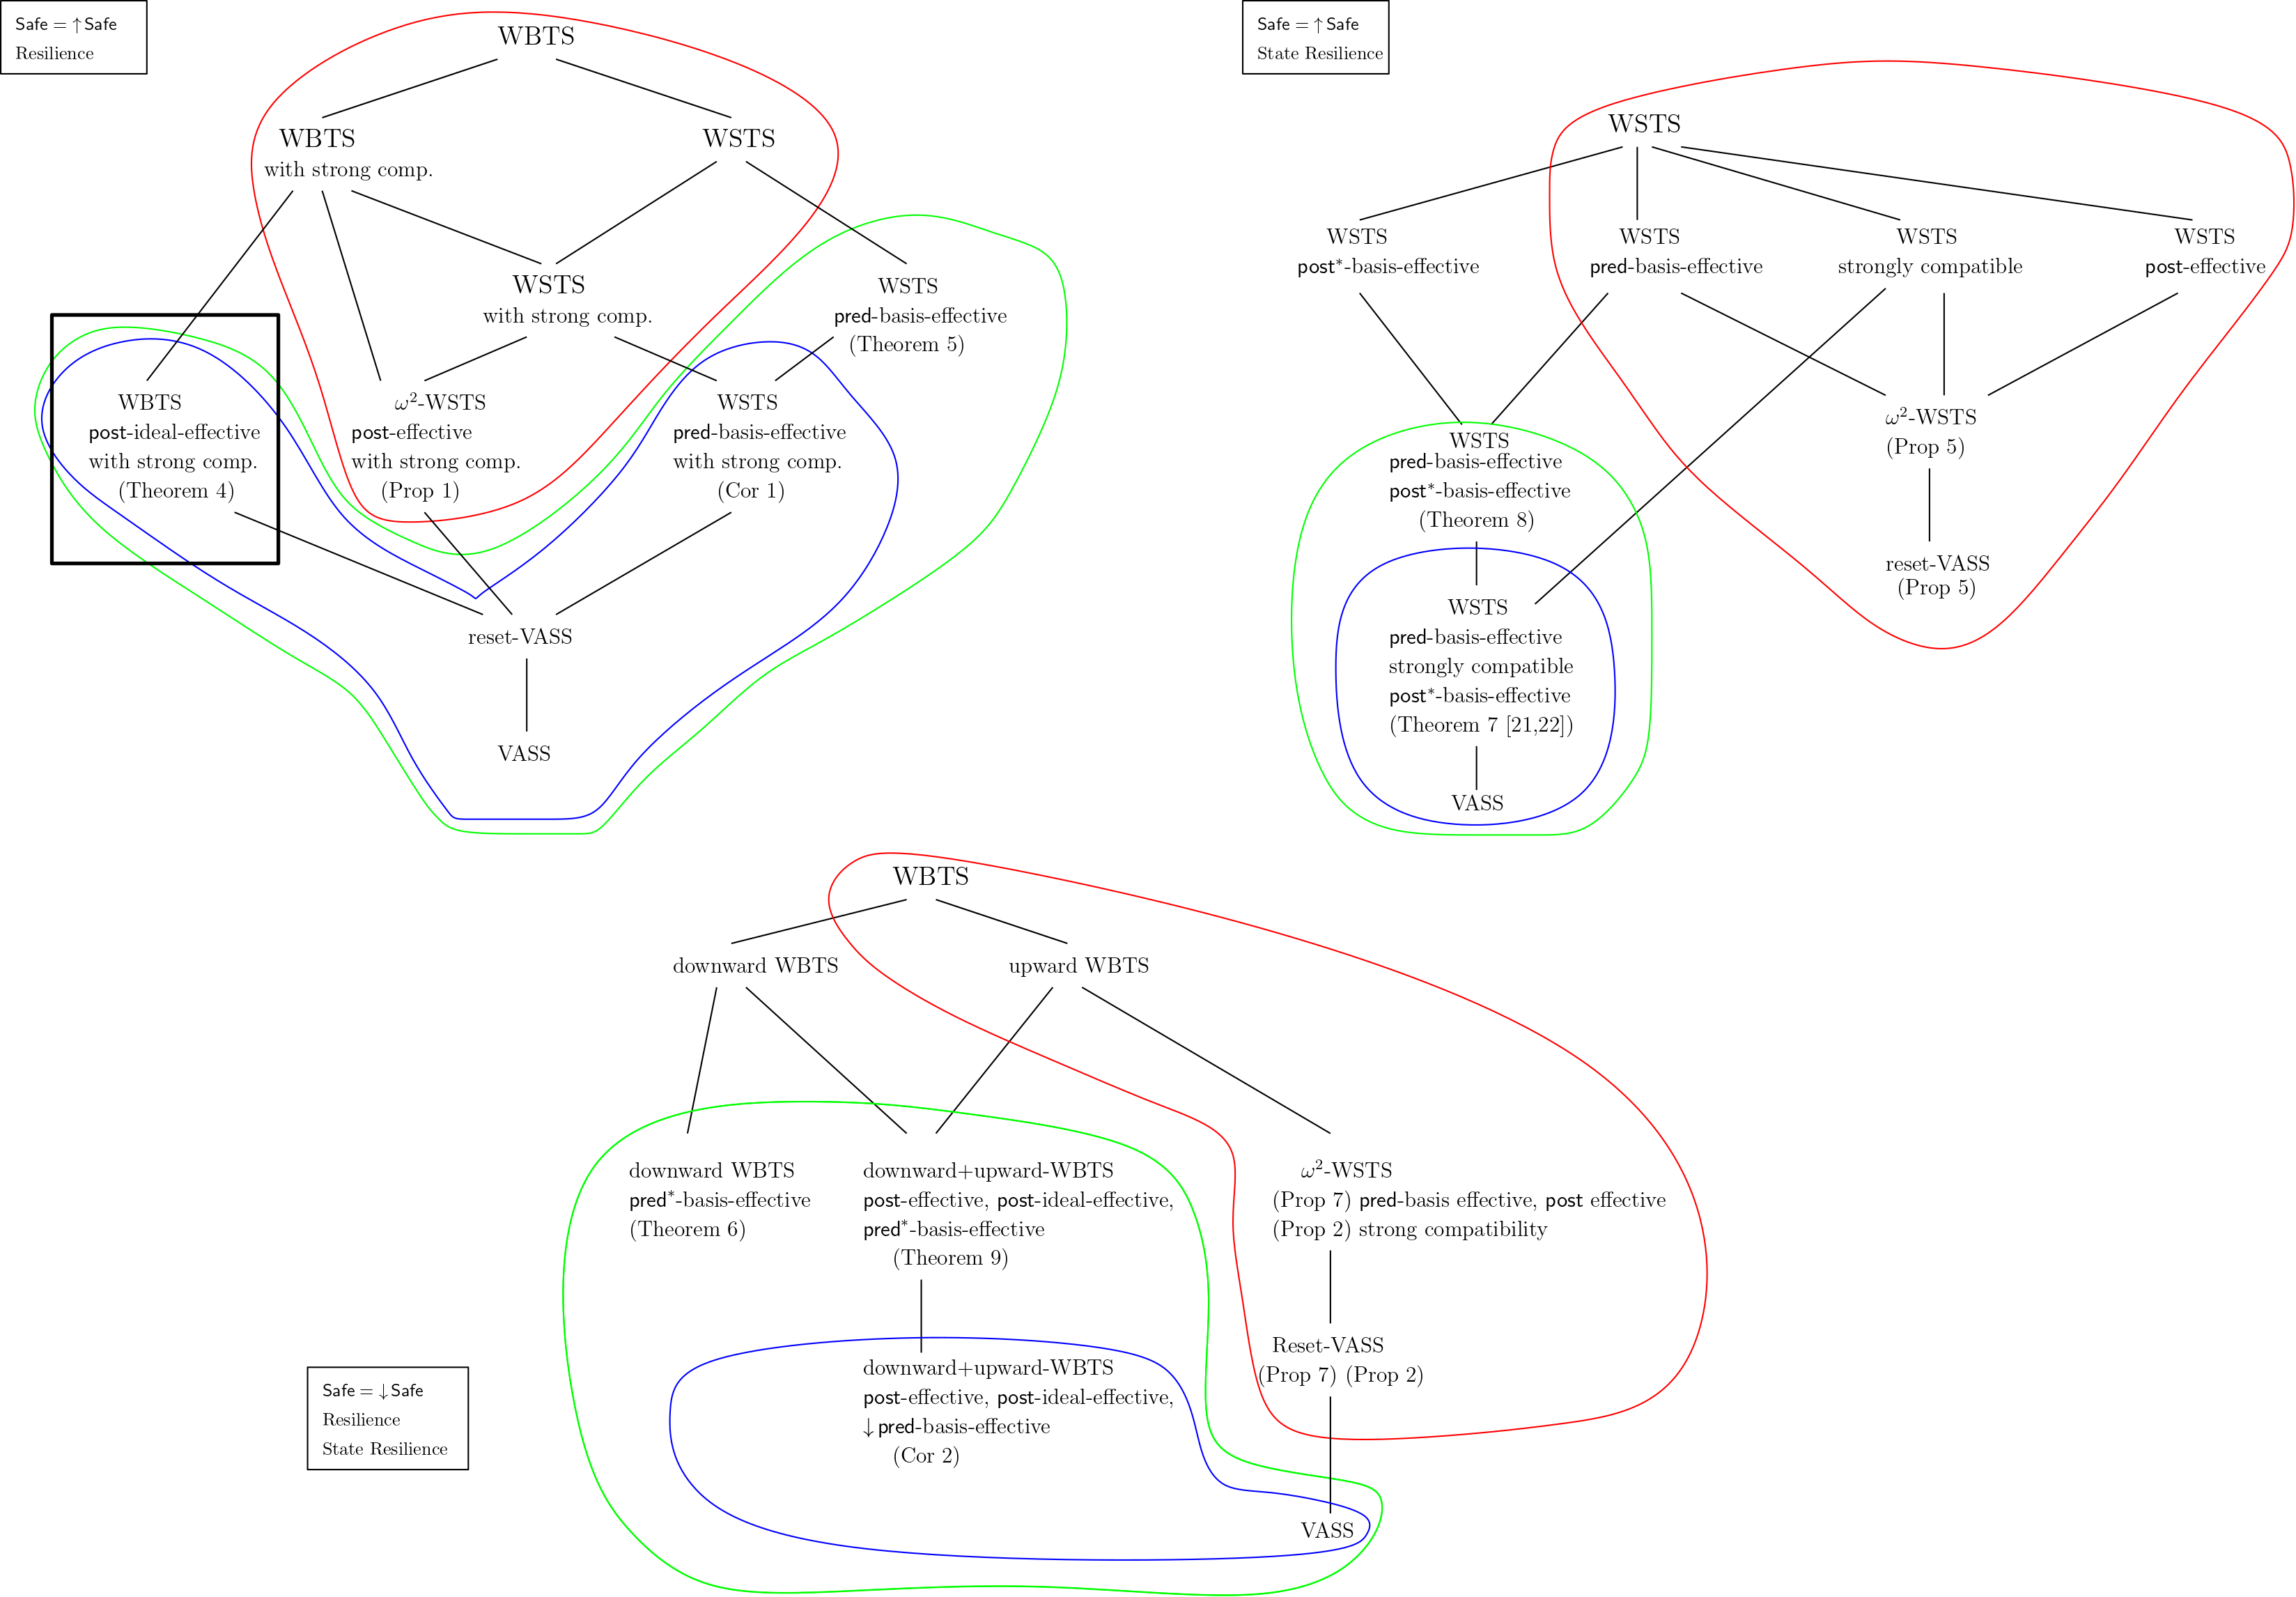
\includegraphics[width=1.00\textwidth]{resultA}
% \caption{Hasse diagram of some classes of transition systems, together with the decidability (in green) or undecidability (in red) of the resilience problems. Decidability of bounded resilience and $k-$resilience variants are indicated in blue.}
	\end{figure}
\end{center}  

    
  \end{frame}
%vvvvvvvvvvvvvvvvvvvvvvvvvvvvvvvvvvvvvvvvvvvvvvvvvvvvvvvvvvvvvvvvvvvvvvvvvv
  \begin{frame}{Result A}
 

  \todo[inline,color=blue!20]{ {\it À l'oral~}   
    Let's delve into [This Result] in particular.
      
   And let's give an intuition behind the proof
      
	...}


  \end{frame}
%vvvvvvvvvvvvvvvvvvvvvvvvvvvvvvvvvvvvvvvvvvvvvvvvvvvvvvvvvvvvvvvvvvvvvvvvvv
  \begin{frame}{Result B}
 
 résultat sur la deuxième figure ?
 on signale juste le thm 8 en passant ?
 
     \todo[inline,color=blue!20]{    Result blabla are consequences of the paper    by Okzan so let's not delve into it.
    ( should still be quite precise about Okzan result and references)}

 
  \end{frame}
%vvvvvvvvvvvvvvvvvvvvvvvvvvvvvvvvvvvvvvvvvvvvvvvvvvvvvvvvvvvvvvvvvvvvvvvvvv
  \begin{frame}{Result C}
 

On On parle des VASS quand Safe downward closed  

  \end{frame}
%vvvvvvvvvvvvvvvvvvvvvvvvvvvvvvvvvvvvvvvvvvvvvvvvvvvvvvvvvvvvvvvvvvvvvvvvvv
  \begin{frame}{Result C}
 
 
   \begin{center}
 	\begin{figure}
 	\hspace{-2.cm}
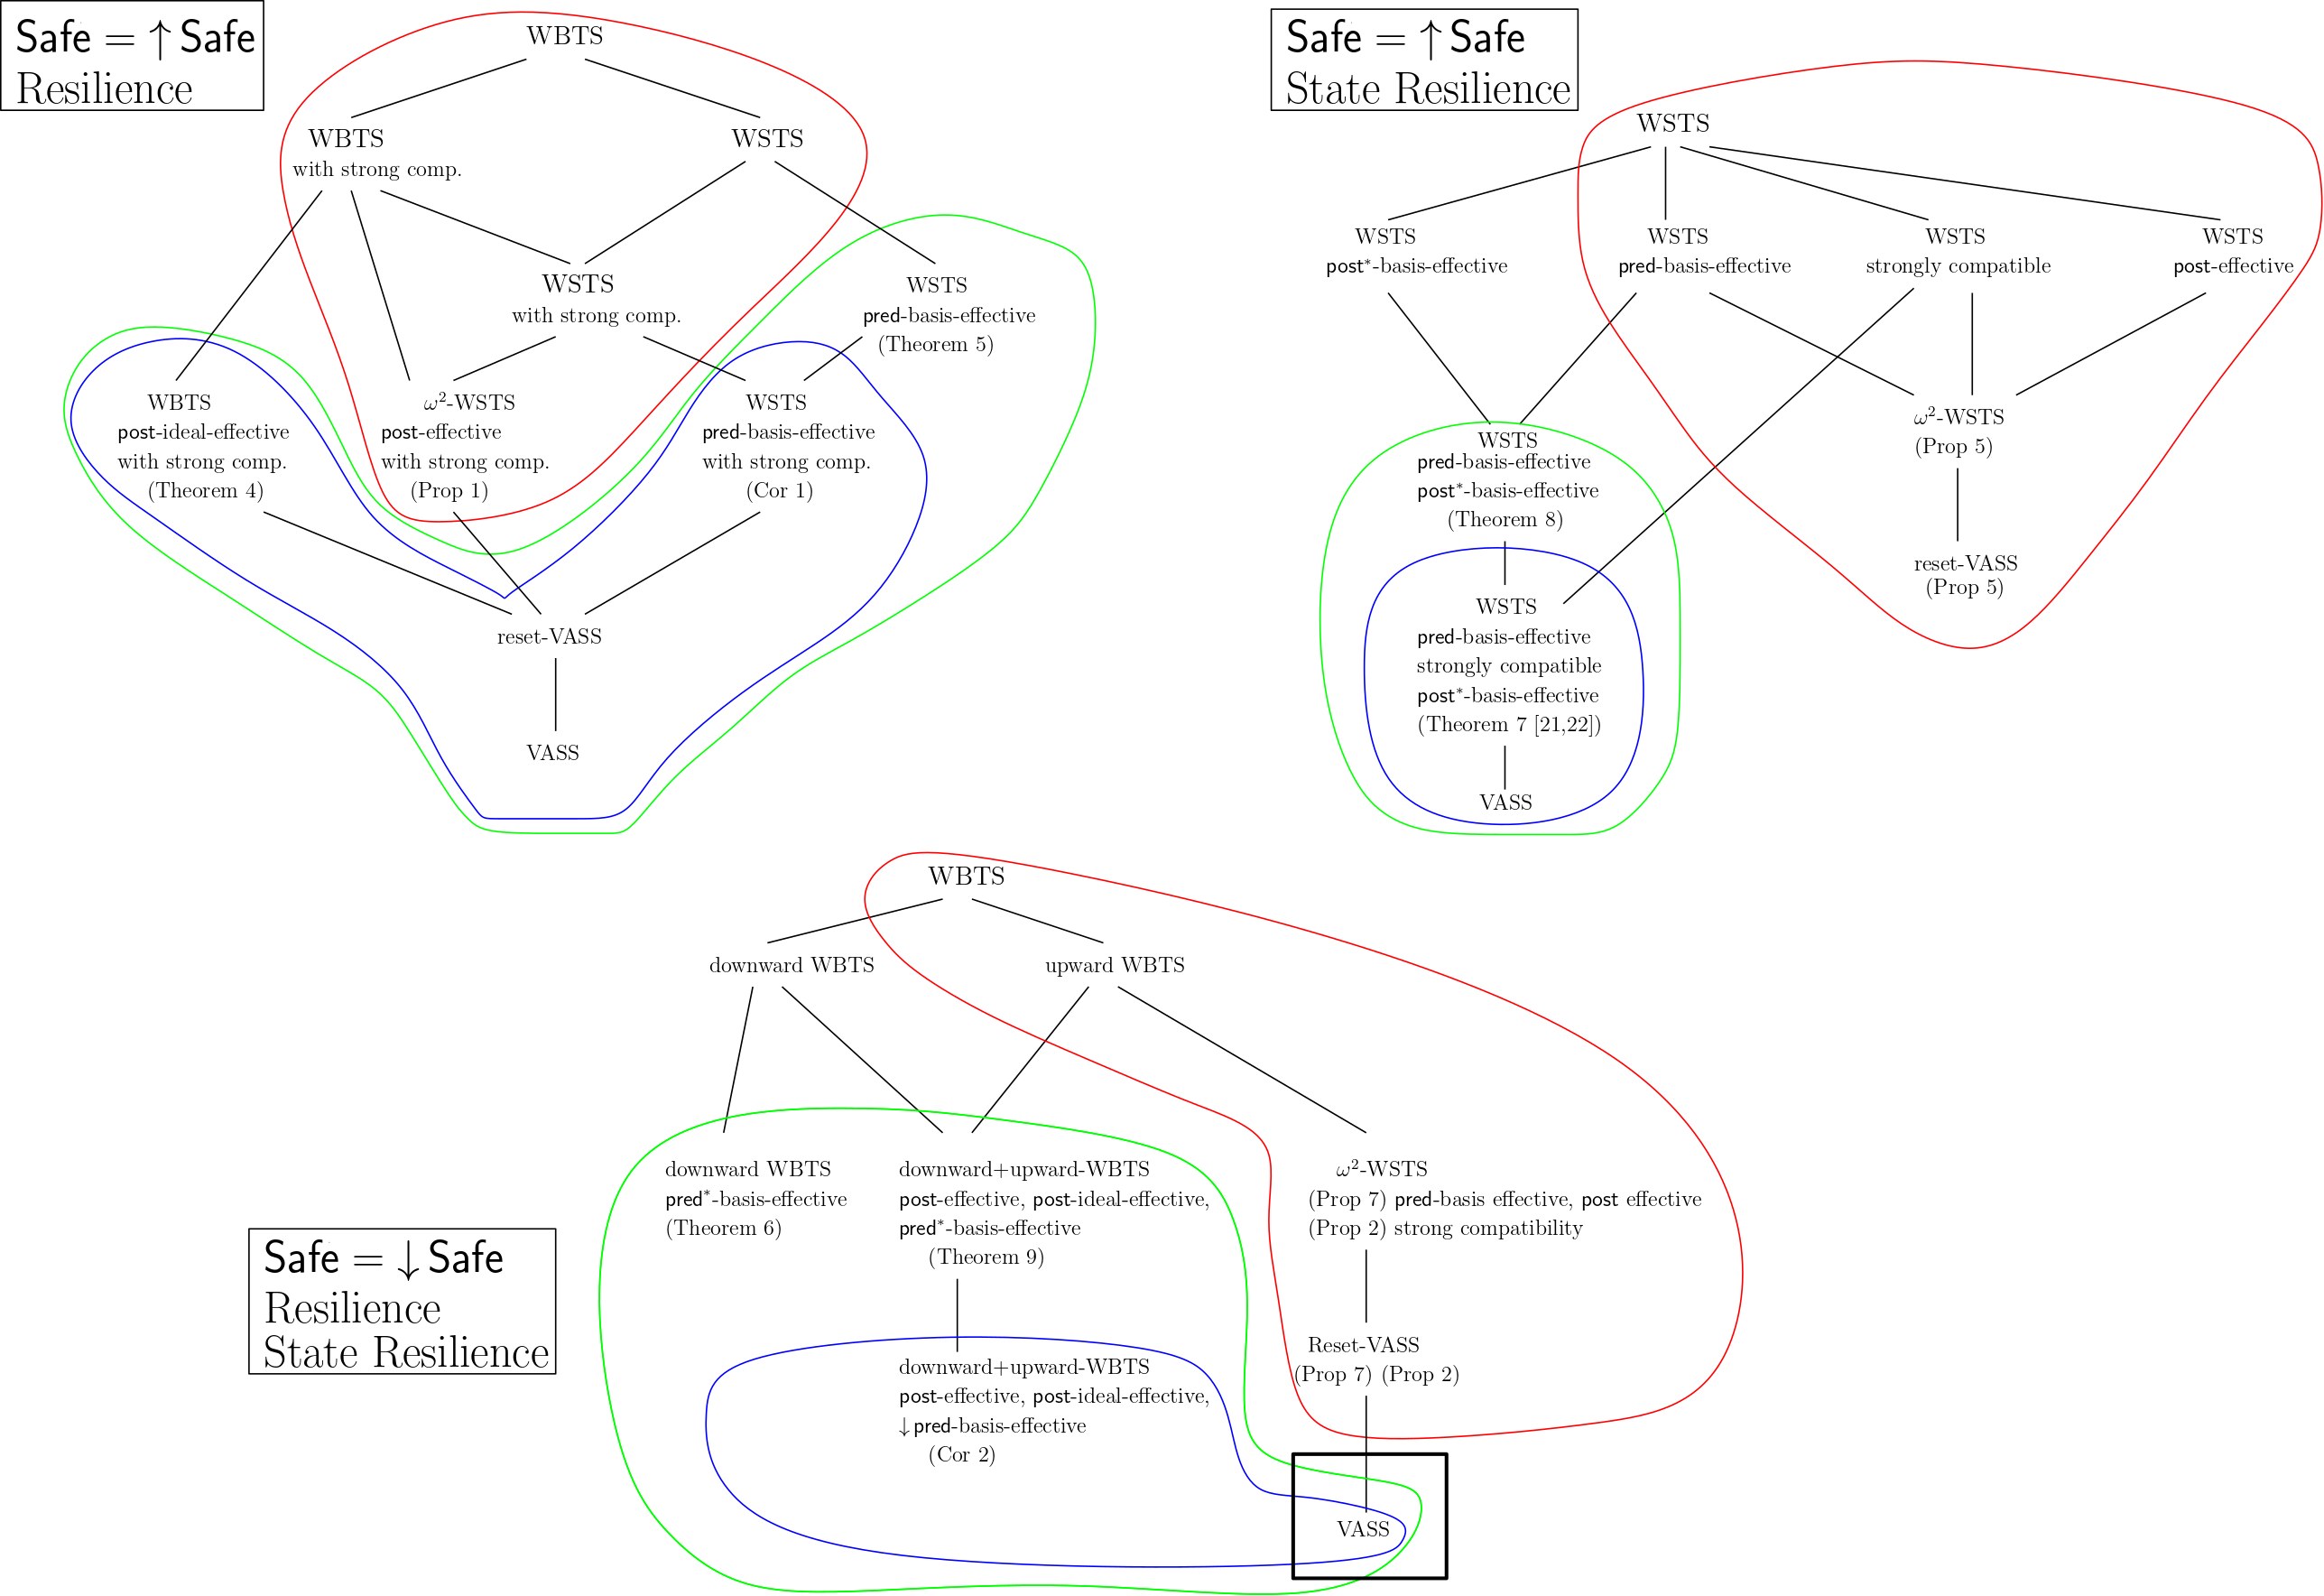
\includegraphics[width=1.00\textwidth]{resultC}
% \caption{Hasse diagram of some classes of transition systems, together with the decidability (in green) or undecidability (in red) of the resilience problems. Decidability of bounded resilience and $k-$resilience variants are indicated in blue.}
	\end{figure}
\end{center}  

  \end{frame}
%vvvvvvvvvvvvvvvvvvvvvvvvvvvvvvvvvvvvvvvvvvvvvvvvvvvvvvvvvvvvvvvvvvvvvvvvvv
  \begin{frame}{Conclusion}
  

How to expand current results ?

- detailed complexity analysis

- controller/environment framework

- other classes of $\Safe / \Bad$


      
  \end{frame}
%vvvvvvvvvvvvvvvvvvvvvvvvvvvvvvvvvvvvvvvvvvvvvvvvvvvvvvvvvvvvvvvvvvvvvvvvvv

 
  
\end{document}
